\documentclass[11pt,a4paper]{jsarticle}
%
\usepackage{amsmath}
\usepackage{emath}
\usepackage{bm}%数式中の太字
\usepackage[dvipdfmx]{graphicx}%図
%
\setlength{\textwidth}{\fullwidth}
\setlength{\textheight}{39\baselineskip}
\addtolength{\textheight}{\topskip}
\setlength{\voffset}{-0.5in}
\setlength{\headsep}{0.3in}
%
\newcommand{\mfo}{\mathfrak{O}\,}  %位相
\newcommand{\st}{\mathrm{s.t.}\,}  %s.t.

\newtheorem{prob}{問題}
\newtheorem{supple}{補足}
\renewcommand{\thesupple}{}%補足について番号を表示しない
\newtheorem{definition}{定義}[subsection]
\newtheorem{theorem}[definition]{定理}%定義から通し番号にする
\newtheorem{proposition}[definition]{命題}
\newtheorem{lemma}[definition]{補題}
\newtheorem{corollary}[definition]{系}
\makeatletter
\def\th@plain{\upshape}
\makeatother

\newtheorem{proof}{証明}
\renewcommand{\theproof}{}
\usepackage{latexsym}
\def\qed{\hfill $\Box$}
%
\begin{document}
%
\setlength{\abovedisplayskip}{3pt} % 上部のマージン
\setlength{\belowdisplayskip}{3pt} % 下部のマージン
%
%
\subsection*{松坂和夫『集合・位相入門』第{6}章$\S${\ }3}
%
\prob
一様同相関係を$\cong$で表すことにする.定義から$(S,d) \cong (S,d),{\ }(S,d) \cong (S',d') \Rightarrow (S',d') \cong (S,d)$は自明.$(S_1,d_1),(S_2,d_2),(S_3,d_3)$を$3$つの距離空間とし,$f_1:S_1 \to S_2,f_2:S_2 \to S_3$とする.そのとき$f_1,f_2$がともに一様連続写像ならば,$f_2 \circ f_1:S_1 \to S_3$も一様連続写像であることを示す.$f_2$は一様連続写像なので
\begin{equation*}
^\forall \epsilon>0, ^\forall x_2,y_2 \in S_2, ^\exists \gamma>0{\ } \st d_2(x_2,y_2)<\gamma \Rightarrow d_3(f_2(x_2),f_2(y_2))<\epsilon
\end{equation*}
が成り立ち,同様に$f_1$は一様連続写像なのでこの$\gamma$に対して
\begin{equation*}
^\forall x_1,y_1 \in S_1, ^\exists \delta>0{\ } \st d_1(x_1,y_1)<\delta \Rightarrow d_2(f_1(x_1),f_1(y_1))<\gamma
\end{equation*}
が成り立つ.以上より
\begin{equation*}
^\forall \epsilon>0, ^\forall x_1,y_1 \in S_1, ^\exists \delta>0{\ } \st d_1(x_1,y_1)<\delta \Rightarrow d_3(f_2(f_1(x_1)),f_2(f_1(y_1)))<\epsilon
\end{equation*}
が成り立つので,$f_2 \circ f_1$が一様連続写像であることが示された.このことから$(S,d) \cong (S',d'),{\ }(S',d') \cong (S'',d'') \Rightarrow (S,d) \cong (S'',d'')$が従う.\qed
%
\prob
一様連続写像の定義よりただちに従う.\qed
%
\prob
$^\forall x,y \in \mathbb{R}^n,{\ }d_{\infty}^{(n)}(x,y) \leq d^{(n)}(x,y) \leq d_{1}^{(n)}(x,y) \leq nd_{\infty}^{(n)}(x,y)$よりただちに従う.\qed
%
\prob
$d$と$d'$が一様同値であることを示す.$f(x)=\frac{x}{1+x}$は単調増加で$\{\frac{x}{1+x} {\ } | {\ }x \in [0,\infty) \}=[0,1)$である.$^\forall \epsilon>0$に対して,$0<\epsilon<1$のときは$\delta=\frac{\epsilon}{1-\epsilon}$とおけば$d(x,y)<\delta \Rightarrow d'(x,y)=\frac{d(x,y)}{1+d(x,y)}<\frac{\delta}{1+\delta}=\epsilon$であり,$\epsilon\geq1$のときは$d'(x,y)<1$より$^\forall \delta>0$について$d(x,y)<\delta \Rightarrow d'(x,y)<\epsilon$であるので,結局$^\forall \epsilon>0, ^\exists \delta>0{\ } \st d(x,y)<\delta \Rightarrow d'(x,y)<\epsilon$が成り立つ.逆についても$d'(x,y)=\frac{d(x,y)}{1+d(x,y)} \Leftrightarrow d(x,y)=\frac{d'(x,y)}{1-d'(x,y)}$より同様に成り立つことを確かめられる.よって$d$と$d'$は一様同値である.
次に$d$と$d''$が一様同値であることを示す.$^\forall \epsilon>0$に対して,$\delta=min\{1,\frac{\epsilon}{p}\}$(ただし$p$は$1$より大きい実数)とおけば,$d(x,y)<\delta \Rightarrow d''(x,y)=min\{1,d(x,y)\}=d(x,y)<\delta=min\{1,\frac{\epsilon}{p}\}<\epsilon$であり,$^\forall \epsilon>0, ^\exists \delta>0{\ } \st d(x,y)<\delta \Rightarrow d''(x,y)<\epsilon$が成り立つ.逆については,$^\forall \epsilon>0$に対して,$\delta=min\{1,\epsilon\}$とおけば,$d''(x,y)<\delta \Rightarrow d(x,y)<\epsilon$であり,$^\forall \epsilon>0, ^\exists \delta>0{\ } \st d''(x,y)<\delta \Rightarrow d(x,y)<\epsilon$が成り立つ.\qed
\begin{figure}[htbp]
 \begin{center}
  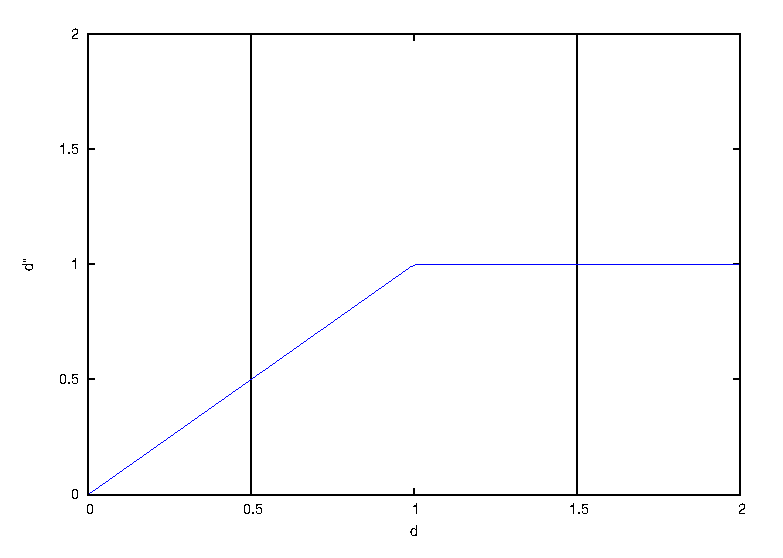
\includegraphics[width=85mm]{graph1.eps}
 \end{center}
\end{figure}
%
\prob
$S=(0,\infty) \subset \mathbb{R}$とする.$d_1$を$\mathbb{R}$におけるEuclid距離関数,$d_2$を$d_2(x,y):=d_1(\frac{1}{x},\frac{1}{y})=\left|\frac{1}{x}-\frac{1}{y}\right|$とする.$d_2$が距離関数になることはただちに示される.また,$\frac{1}{x}$の連続性から$d_1$と$d_2$が同値であることは明らかである.$^\exists \epsilon>0, ^\forall \delta>0$に対して,$^\exists x,y \in S$を$\displaystyle x \leq -\frac{\delta}{2p}+\frac{1}{2\epsilon}\sqrt{\frac{\epsilon^2\delta^2}{p^2}+\frac{4\epsilon\delta}{p}}(>0),y=x+\frac{\delta}{p}$(ただし$p$は$1$より大きい実数)を満たすように取る.このとき$|y-x|=\frac{\delta}{p}<\delta$であり
\begin{equation*}
\left| \frac{1}{y}-\frac{1}{x} \right|=\frac{\frac{\delta}{p}}{(x+\frac{\delta}{p})x} \geq …=\epsilon
\end{equation*}
が成り立つので,$^\exists\epsilon>0{\ }\st ^\forall\delta>0, ^\exists x,y \in S {\ }\st d_1(x,y)<\delta \cap d_2(x,y) \geq \epsilon$が成り立ち,$d_1$と$d_2$は一様同値でないことが示された.\qed
\supple
ここで,$\epsilon$の取り得る値は関数($\frac{1}{x}$)に対して決まり,この場合,任意の正の実数を取る.また,$f:\mathbb{R} \ni x \mapsto \frac{1}{x} \in \mathbb{R}$とおけば,$d_2(x,y)=d_1(f(x),f(y))$と書けるので,この例で示したことは$f:(\mathbb{R},d_1) \to (\mathbb{R},d_1)$が一様連続でないことと同値である.よって同様にして$\mathbb{R} \to \mathbb{R}$の一様連続でない関数を用いて,Euclid距離と同値だが一様同値ではない距離の例を作ることができる.
%
\prob
$f:\mathbb{R}\times\mathbb{R}\ni(x,y)\mapsto x+y \in \mathbb{R}$が一様連続写像であることを示す.$^\forall \epsilon>0$に対して$\delta=\frac{\epsilon}{2}$とおく.$d^{(2)}((x_1,y_1),(x_2,y_2))<\delta=\frac{\epsilon}{2}$であるとすると$d^{(1)}(x_1,x_2)^2+d^{(1)}(y_1,y_2)^2<\frac{\epsilon^2}{4}$となるので,$d^{(1)}(x_1,x_2)<\frac{\epsilon}{2},d^{(1)}(y_1,y_2)<\frac{\epsilon}{2}$が成り立つ.よって,$d^{(1)}(x_1+y_1,x_2+y_2)=|(x_2+y_2)-(x_1+y_1)|=|(x_2-x_1)+(y_2-y_1)|\leq|x_2-x_1|+|y_2-y_1|=d^{(1)}(x_1,x_2)+d^{(1)}(y_1,y_2)<\epsilon$が成り立つので,$f$は一様連続写像である.\\
次に$g:\mathbb{R}\times\mathbb{R}\ni(x,y)\mapsto xy \in \mathbb{R}$が一様連続写像でないことを示す.$^\exists \epsilon>0, ^\forall \delta>0$に対して,$^\exists (x_1,y_1),(x_2,y_2) \in \mathbb{R}^2$を$\displaystyle x_1+y_1 \geq \frac{p\epsilon}{\delta},x_2=x_1+\frac{\delta}{p},y_2=y_1+\frac{\delta}{p}$(ただし$p$は$\sqrt{2}$より大きい実数)を満たすように取る.このとき$d^{(2)}((x_1,y_1),(x_2,y_2))^2=d^{(1)}(x_1,x_2)^2+d^{(1)}(y_1,y_2)^2=\frac{2\delta^2}{p^2}<\delta^2$であり,このとき$d^{(1)}(x_1y_1,x_2y_2)=|x_2y_2-x_1y_1|=\frac{\delta}{p}(x_1+y_1)+\frac{\delta^2}{p^2} \geq \epsilon+\frac{\delta^2}{p^2}>\epsilon$
が成り立つので,$g$は一様連続写像でないことが示された.\qed
\begin{figure}[htbp]
 \begin{center}
  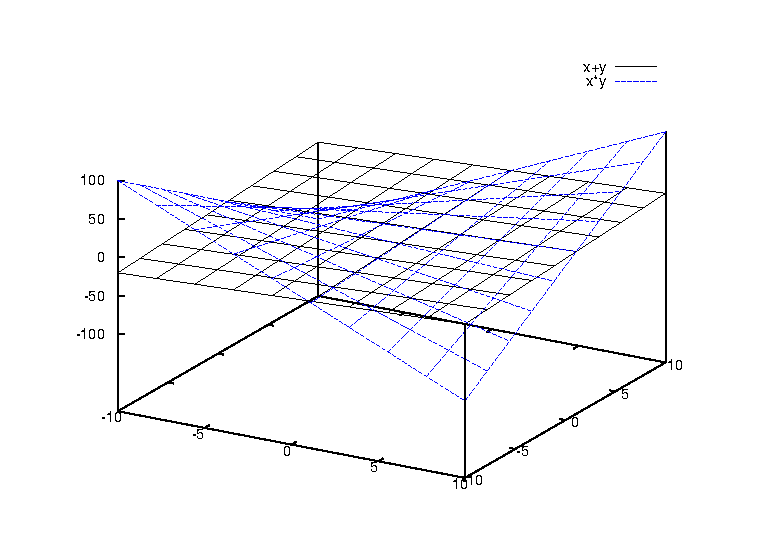
\includegraphics[width=85mm]{graph2.eps}
 \end{center}
\end{figure}
%
\prob
$\mathbb{R}$のEuclid距離関数を$d^{(1)}$と表すことにする.$S\times S$上の$2$点$(x_1,y_1),(x_2,y_2)$を取る.$S\times S$に直積距離を入れて,その距離関数を$d'$で表せば$d'((x_1,y_1),(x_2,y_2))^2=d(x_1,x_2)^2+d(y_1,y_2)^2$が成り立つ.$^\forall \epsilon>0$に対して$\delta=\frac{\epsilon}{2}$とおく.$d'((x_1,y_1),(x_2,y_2))<\delta$であるとすると$d(x_1,x_2)<\frac{\epsilon}{2},d(y_1,y_2)<\frac{\epsilon}{2}$が成り立つ.よって,$d^{(1)}(d(x_1,y_1),d(x_2,y_2)) \leq d^{(1)}(d(x_1,y_1),d(x_2,y_1))+d^{(1)}(d(x_2,y_1),d(x_2,y_2)) = |d(x_2,y_1)-d(x_1,y_1)|+|d(x_2,y_2)-d(x_2,y_1)| \leq d(x_1,x_2)+d(y_1,y_2) < \epsilon$が成り立つので$d$一様連続写像であることが示された.ただし最後の式変形において$d^{(1)}$の三角不等式と$d$の三角不等式を順次用いた.\qed
\supple
$\mathbb{R}$に$d^{(1)}$と一様同値な距離が入っている場合,$d$は一様連続写像となる.これは以下のように示される.$d^{(1)}$と一様同値な距離を$d_{e}$とおく.このとき
\begin{equation*}
^\forall x,y \in \mathbb{R}, ^\forall\epsilon >0, ^\exists\gamma>0,{\ }\st d^{(1)}(x,y)< \gamma \Rightarrow d_{e}(x,y) < \epsilon
\end{equation*}
が成り立つ.一方,問題で示したことから,この$\gamma$について
\begin{equation*}
^\forall x_1,y_1,x_2,y_2 \in S, ^\exists \delta>0 {\ } \st d'((x_1,y_1),(x_2,y_2))<\delta \Rightarrow d^{(1)}(d(x_1,y_1),d(x_2,y_2)) < \gamma
\end{equation*}
が成り立つので,以上より
\begin{equation*}
^\forall x_1,y_1,x_2,y_2 \in S, ^\forall \epsilon>0, ^\exists \delta>0 {\ } \st d'((x_1,y_1),(x_2,y_2))<\delta \Rightarrow d_e(d(x_1,y_1),d(x_2,y_2)) < \epsilon
\end{equation*}
が成り立つ.よって,$d:S \times S \to (\mathbb{R},d_e)$は一様連続写像である.この証明からわかるように,$\mathbb{R}$にEuclid距離と一様同値でない距離が入っている場合$d$は一様連続写像であるとは限らない.例えば,P.235第6章$\S${\ }$1$例$2$のような病的な距離が入っているとき,$d$は一様連続写像ではない.
%
\prob
$(S,d),(S',d')$を$2$つの一様同相な距離空間とし,$(S,d)$は完備であるとする.また,$f:S \to S'$とする.このとき$(S',d')$も完備であることを示す.$S'$の任意のCauchy列$(a_n)_{n \in \mathbb{N}}$を取る.$(a_n)_{n \in \mathbb{N}}$はCauchy列であることから
\begin{equation*}
^\forall \gamma>0, ^\exists n_0 \in \mathbb{N}{\ }\st ^\forall m,n \in \mathbb{N},m>n_0,n>n_0,d'(a_m,a_n)<\gamma
\end{equation*}
が成り立つ.また$f^{-1}$が一様連続写像であることから
\begin{equation*}
^\forall \epsilon>0, ^\exists \gamma>0{\ }\st d'(a_m,a_n)<\delta \Rightarrow d(f^{-1}(a_m),f^{-1}(a_n))<\epsilon
\end{equation*}
が成り立つ.この$\delta$に対して第一式で特に$\gamma=\delta$とすれば第二式より
\begin{equation*}
^\forall \epsilon>0, ^\exists n_0 \in \mathbb{N}{\ }\st ^\forall m,n \in \mathbb{N},m>n_0,n>n_0,d(f^{-1}(a_m),f^{-1}(a_n))<\epsilon
\end{equation*}
が成り立つので,$((f^{-1}(a_n))_{n \in \mathbb{N}})$は$S$におけるCauchy列である.$S$は完備であるので,$((f^{-1}(a_n))_{n \in \mathbb{N}})$は$S$内の点に収束する.$((f^{-1}(a_n))_{n \in \mathbb{N}})$の極限を$A_S$とおく.$f$は特に連続写像であるので,P.240第6章{\S}{\ }1定理3(ii)より,$\displaystyle \lim_{n \to \infty} f(f^{-1}(a_n))=\lim_{n \to \infty} a_n=f(A_S)$が成り立つので,結局$S'$の任意のCauchy列$(a_n)_{n \in \mathbb{N}}$が収束することが示された.よって$(S',d')$も完備である.\qed
%
\prob
$M$が$S$の閉集合のとき,$S$の任意のCauchy列$(a_n)_{n \in \mathbb{N}}$を取れば,$S$が完備であるので$(a_n)_{n \in \mathbb{N}}$は$S$内の点に収束するが,その極限を$a$とおけばP.239第$6$章$\S${\ }$1$定理$2$より$a \in \overline{M}=M$となり,$M$は完備であることが示された.また$M$が$S$の閉集合でなければ,一般に$S$のCauchy列で$M$に収束しないものが存在する.よって$M$は完備でない.\qed
%
\prob(a)
$S_1 \times S_2$の点列$((a_n^{(1)},a_n^{(2)}))_{n \in \mathbb{N}}$がCauchy列であるとき,$^\forall \epsilon>0, ^\exists n_0 \in \mathbb{N}{\ }\st ^\forall m,n \in \mathbb{N},m>n_0,n>n_0,d(a_m,a_n)<\epsilon$が成り立つ.ここで,$\displaystyle d(a_m,a_n)<\epsilon \Leftrightarrow \sum_{i=1}^2 d_i(a_m^{(i)},a_n^{(i)})^2<\epsilon^2$であるので,$i=1,2$について$d_i(a_m^{(i)},a_n^{(i)})<\epsilon$が成り立つ.よって$(a_n^{(1)})_{n \in \mathbb{N}},(a_n^{(2)})_{n \in \mathbb{N}}$はそれぞれ$S_1,S_2$のCauchy列である.逆に$(a_n^{(1)})_{n \in \mathbb{N}},(a_n^{(2)})_{n \in \mathbb{N}}$がそれぞれ$S_1,S_2$のCauchy列であるとき,$^\forall \epsilon>0$に対して,
\begin{eqnarray*}
^\exists a \in \mathbb{N}{\ }\st ^\forall m_a,n_a \in \mathbb{N},m_a>a,n_a>a,d_1(a_{m_a}^{(1)},a_{n_a}^{(1)})<\frac{\epsilon}{\sqrt{2}} \\
^\exists b \in \mathbb{N}{\ }\st ^\forall m_b,n_b \in \mathbb{N},m_b>b,n_b>b,d_1(a_{m_b}^{(2)},a_{n_b}^{(2)})<\frac{\epsilon}{\sqrt{2}}
\end{eqnarray*}
が成り立つ.$n_0=max\{a,b\}$とおけば,上の二式より
\begin{equation*}
^\forall \epsilon>0, ^\exists n_0 \in \mathbb{N}{\ }\st ^\forall m,n \in \mathbb{N},m>n_0,n>n_0,d(a_m,a_n)^2=\sum_{i=1}^2 d_i(a_m^{(i)},a_n^{(i)})^2<\epsilon^2
\end{equation*}
が成り立つ.よって$S_1 \times S_2$の点列$((a_n^{(1)},a_n^{(2)}))_{n \in \mathbb{N}}$はCauchy列である.\\
(b){\ }(a)よりただちに従う.\qed
%
\prob
P.257第6章{\S}{\ }3定理8と問題10(b)よりただちに従う.\qed
%
\prob
$(a_n)_{n \in \mathbb{N}}$はCauchy列であるので,$^\forall\epsilon>0, ^\exists n_1 \in \mathbb{N}{\ } \st ^\forall m,n \in \mathbb{N}, m>n_1,n>n_1,d(a_m,a_n)<\frac{\epsilon}{2}$が成り立つ.また$(a_n)_{n \in \mathbb{N}}$は$a$に収束する部分列$(a_{i_n})_{n \in \mathbb{N}}$を含むので,$^\forall\epsilon>0, ^\exists n_2 \in \mathbb{N}{\ } \st ^\forall i_n>n_2,d(a_{i_n},a)<\frac{\epsilon}{2}$が成り立つ.ここで$max\{n_1,n_2\}=n_0$とおけば,特に$^\forall\epsilon>0, ^\forall i_n>n_0,d(a_{i_n},a)<\frac{\epsilon}{2}$が成り立つ.この条件を満たす$i_n$を$1$つ取って,それを$i_k$とおく.この$i_k$を用いれば,$^\forall\epsilon>0, ^\forall n \in \mathbb{N}, n>n_1,d(a_n,a) \leq d(a_n,a_{i_k})+d(a_{i_k},a)<\frac{\epsilon}{2}+\frac{\epsilon}{2}=\epsilon$が成り立つので,$(a_n)_{n \in \mathbb{N}}$自身が$a$に収束することが示された.
\qed
%
\prob
P.260第6章{\S}{\ }3定理10より,ある距離空間$(S,d)$が全有界であるための必要十分条件は$S$の任意の点列がCauchy列を部分列として含むことであるので,後者の性質が一様同相写像の元で保存されることを示すことにする.$(S,d),(S',d')$を$2$つの一様同相な距離空間とし,$(S,d)$の任意の点列がCauchy列を部分列として含むとする.また,$f:S \to S'$とする.このとき$(S',d')$の任意の点列がCauchy列を部分列として含むことを示す.$S'$の任意の点列$(a_n)_{n \in \mathbb{N}}$を取る.$(f^{-1}(a_n))_{n \in \mathbb{N}}$は$S$における点列であるので,Cauchy列$(f^{-1}(a_{n'}))_{n \in \mathbb{N}}:=(f^{-1}(a_{i_n}))_{n \in \mathbb{N}}$を部分列として含む.$(f^{-1}(a_{n'}))_{n \in \mathbb{N}}$はCauchy列であるので
\begin{equation*}
^\forall \gamma>0, ^\exists n_0 \in \mathbb{N}{\ }\st ^\forall m,n \in \mathbb{N},m>n_0,n>n_0,d(f^{-1}(a_{m'}),f^{-1}(a_{n'}))<\gamma
\end{equation*}
が成り立つ.ここで,$f$は一様連続写像であるので
\begin{equation*}
^\forall \epsilon>0, ^\exists \delta>0{\ }\st d'(f^{-1}(a_{m'}),f^{-1}(a_{n'}))<\delta \Rightarrow d(a_{m'},a_{n'})<\epsilon
\end{equation*}
が成り立つ.この$\delta$に対して第一式で特に$\gamma=\delta$とすれば第二式より
\begin{equation*}
^\forall \epsilon>0, ^\exists n_0 \in \mathbb{N}{\ }\st ^\forall m,n \in \mathbb{N},m>n_0,n>n_0,d(a_{m'},a_{n'})=d(a_{i_m},a_{i_n})<\epsilon
\end{equation*}
が成り立つので,$(S',d')$の任意の点列がCauchy列を部分列として含むことが示された.\qed
%
\prob
(コンパクト性を用いた証明){\ }
$\mathbb{R}^n$の任意の有界な部分集合を$M$とする.このとき,$\overline{M}$は$\mathbb{R}$の有界な閉集合となるのでコンパクトである.$^\forall\epsilon>0$に対して$\mathfrak{U}:=\{B(x,\frac{\epsilon}{p}){\ }|{\ }x \in \overline{M}\}$(ただし$p$は$1$より大きい実数)は$\overline{M}$の$\epsilon$被覆となるので,$\mathfrak{U}$から適当な有限部分集合$\mathfrak{U}_0:=\{B(x_i,\frac{\epsilon}{p}){\ }|{\ }x_i \in \overline{M}{\ }(i=1,2,\cdots,n)\}$を取り出せば,$\mathfrak{U}_0$は$\overline{M}$の有限な$\epsilon$被覆となる.ここで,$\mathfrak{U}_0$は$M$の有限な$\epsilon$被覆でもあるので,$M$は全有界であることが示された.
\qed\\
(構成的な証明){\ }
P.248第$6$章$\S${\ }$2$補題$1$より,$^\forall a \in \mathbb{R}^n, ^\exists R>0{\ }\st M \subsetneq B(a,R)$が成り立つので,$a$を中心とした$1$辺$R$の$n$次元”立方体”を$C(a,R)$とおけば,$M \subsetneq C(a,R)$が成り立つ.ここで,$1$辺$r$の$n$次元”立方体”を$C(r)$と書くことにすると,$^\forall\epsilon>0$に対して,$\delta(C(\frac{\epsilon}{\sqrt{n}p}))=\frac{\epsilon}{p}<\epsilon$(ただし$p$は$1$より大きい実数)である.$C(a,R)$は$C(\frac{\epsilon}{\sqrt{n}p})$を$\left( \left[ \frac{\sqrt{n}pR}{\epsilon} \right]+1 \right) ^n(<\infty)$(ただし[{\ }]はガウス記号)個並べることで被覆される.よって$C(a,R)$は全有界となるので,特に$M$は全有界であることが示された.
\qed
%
\prob
$S$が全有界であるとき$^\forall\epsilon>0$に対して$S$の有限な$\epsilon$網が存在することは,P.259第$6$章$\S${\ }$3$定理$9$の証明中で示されている.逆に$^\forall\epsilon>0$に対して$S$の有限な$\epsilon$網が存在する存在するとき,$\frac{\epsilon}{2p}$(ただし$p$は$1$より大きい実数)網を$M$とおけば,$\{B(x,\frac{\epsilon}{2p}){\ }|{\ }x \in M\}$は$S$の有限被覆となり,$^\forall\epsilon>0$に対して$\delta(B(x,\frac{\epsilon}{2p}))=\frac{\epsilon}{p}<\epsilon$となるので,有限な$\epsilon$被覆である.よって$S$は全有界である.
\qed
%
\prob
$S,S_1,S_2$の距離をそれぞれ$d_S,d_{S_1},d_{S_2}$とおく.$S$が全有界であるとき,$^\forall\epsilon>0$に対して有限な$\epsilon$網が存在するので,これを$M$とおけば,$^\forall (x_1,x_2) \in S$に対して$d_S((x_1,x_2),M)<\epsilon$が成り立つ.このとき,$d_S((x_1,x_2),M)=inf\{d_S((x_1,x_2),m){\ }|{\ }m \in M\}$を与える$m$を$m_0$とおけば($M$は有限部分集合であるのでこのような$m_0$は存在する),$d_S((x_1,x_2),m_0)=\sqrt{d_{S_1}(x_1,pr_1(m_0))^2+d_{S_2}(x_2,pr_2(m_0))^2}<\epsilon$であるので,結局
\begin{eqnarray*}
^\forall\epsilon>0, ^\forall x_1 \in S_1, ^\exists pr_1(m_0) \in pr_1(M) {\ } \st d_{S_1}(x_1,pr_1(m_0))<\epsilon\\
^\forall\epsilon>0, ^\forall x_2 \in S_2, ^\exists pr_2(m_0) \in pr_2(M) {\ } \st d_{S_2}(x_2,pr_2(m_0))<\epsilon
\end{eqnarray*}
が成り立つ.よって,$pr_1(M),pr_2(M)$はそれぞれ$S_1,S_2$の有限な$\epsilon$網となるので,$S_1,S_2$は全有界である.逆に$S_1,S_2$が全有界であるとき,$^\forall\epsilon>0$に対してそれぞれ有限な$\frac{\epsilon}{\sqrt{2}}$網が存在するので,これを$M_1,M_2$とおけば,$^\forall (x_1,x_2) \in S$に対して$d_{S_1}(x_1,M_1)<\frac{\epsilon}{\sqrt{2}},d_{S_2}(x_2,M_2)<\frac{\epsilon}{\sqrt{2}}$が成り立つ.このとき$i=1,2$に対して,$d_{S_i}(x_i,M_i)=inf\{d_{S_i}(x_i,m_i){\ }|{\ }m_i \in M_i\}$を与える$m_i$を$m_0^{(i)}$とおけば($M$は有限部分集合であるのでこのような$m_0^{(i)}$は存在する),$d_S((x_1,x_2),(m_0^{(1)},m_0^{(2)}))=\sqrt{d_{S_1}(x_1,m_0^{(1)})^2+d_{S_2}(x_2,m_0^{(2)})^2}<\epsilon$であるので,結局
\begin{equation*}
^\forall\epsilon>0, ^\forall (x_1,x_2) \in S, ^\exists (m_1,m_2) \in M_1 \times M_2 {\ } \st d_S((x_1,x_2),(m_0^{(1)},m_0^{(2)}))<\epsilon
\end{equation*}
が成り立つ.よって$M_1 \times M_2$は$S$の有限な$\epsilon$網となるので,$S$は全有界である.
\qed
\supple
例えば$\mathbb{R}^2$において,$([1,2]\times[1,2]) \cup ([3,4]\times[3,4]) \neq ([1,2] \cup [3,4]) \times ([1,2] \cup [3,4])$であることに注意.
%
%
\end{document}